\documentclass[t,compress,10pt,xcolor=dvipsnames]{beamer}

\usepackage{amsmath}
\newtheorem{mydef}{Definici\'on}
\usepackage{lmodern}
\usepackage[labelformat=empty,labelsep=none]{subfig}
\usepackage{caption}
\usepackage{float}
\usepackage{wrapfig}
\usepackage{algorithm}


%\makeatletter
%\renewcommand{\ALG@name}{Algoritmo}
%\renewcommand{\listalgorithmname}{List of \ALG@name s}
%\renewcommand{\algorithmicrequire}{Par\'ametros de entrada:}
%\makeatother


\DeclareMathOperator*{\argmax}{arg\,max}
\DeclareMathOperator*{\argmin}{arg\,min}

\newcommand*\oldmacro{}%
\let\oldmacro\insertshorttitle% 
\renewcommand*\insertshorttitle{%
\oldmacro\hfill%
\insertframenumber\,/\,\inserttotalframenumber}

\definecolor{UniDunkel}{RGB}{73,142,137}
\definecolor{UniHell}{RGB}{142,184,182}

\setbeamertemplate{blocks}[rounded][shadow=true]
\setbeamercolor{structure}{fg=UniDunkel}

\setbeamercolor{block body}{parent=normal text,use=block title,bg=block title.bg!10!bg}
\setbeamercolor{block body alerted}{parent=normal text,use=block title alerted,bg=block title alerted.bg!10!bg}
\setbeamercolor{block body example}{parent=normal text,use=block title example,bg=block title example.bg!10!bg}

\setbeamercolor*{palette primary}{use=structure,fg=white,bg=UniDunkel!115}
\setbeamercolor*{palette secondary}{use=structure, fg=UniHell,  bg=UniHell}
\setbeamercolor*{palette tertiary}{use=structure,fg=white,bg=UniDunkel!115}
\setbeamercolor*{palette quaternary}{fg=Orange}

\setbeamercolor*{sidebar}{use=structure,bg=structure.fg}
\setbeamercolor*{palette sidebar primary}{use=structure,fg=structure.fg!10}
\setbeamercolor*{palette sidebar secondary}{fg=white}
\setbeamercolor*{palette sidebar quaternary}{fg=white}
\setbeamercolor*{titlelike}{parent=palette primary}

\setbeamercolor*{fine separation line}{}

\setbeamercolor{block title}{use=structure,fg=white,bg=structure.fg!0!red}
\setbeamercolor{block title alerted}{use=alerted text,fg=white,bg=alerted text.fg!0!white}
\setbeamercolor{block title example}{use=example text,fg=white,bg=example text.fg!0!white}

\useoutertheme{miniframes}
\useinnertheme{circles}
\setbeamertemplate{footline}[frame number]

\beamertemplatenavigationsymbolsempty

\usepackage{textpos} 
\usepackage{mathptmx}
\usepackage{anyfontsize}
\usepackage{t1enc}
\usepackage{multicol}
\usepackage{lmodern}

%\addtobeamertemplate{frametitle}{}{%
%\begin{textblock*}{100mm}(11cm,-1cm)
%	\includegraphics[height=1cm]{logo.png}
%\end{textblock*}}

%\titlegraphic{
%	\includegraphics[width=5cm]{backg}
%}

\title{\textbf{Agrupamiento y clasificaci\'on en la recuperaci\'on de informaci\'on en la web}}

%\author{Integrantes:\\
%	Marcos Manuel Tirador del Riego\\ 
%	Laura Victoria Riera P\'erez\\
%	Leandro Rodr\'iguez Llosa}
%\institute{Ciencias de la computaci\'on}
\date{}

%\usepackage{tikz}
%\titlegraphic { 
%	\begin{tikzpicture}[remember picture]
%		\node[left=0.2cm] at (current page.30){
%			\includegraphics[width=10cm]{backg}
%		};
%	\end{tikzpicture}
%}

\setbeamercolor{block body}{bg=Emerald,fg=Emerald}



\begin{document}
	
	\begin{frame}
		\begin{center}
			\begin{block}{}
				\centering
				\Large\textcolor{white}{\textbf{Agrupamiento y clasificaci\'on en la recuperaci\'on de informaci\'on en la web}}
			\end{block}
		
		\vspace{0.5em}
		
\includegraphics[width=3cm]{clustering.jpg}
		
		\vspace{0.5em}
		\footnotesize
		Integrantes:\\
			Marcos Manuel Tirador del Riego\\ 
			Laura Victoria Riera P\'erez
		
		\vspace{0.7em}
		\tiny	
		Tercer año. Ciencias de la computaci\'on. Universidad de La Habana. Cuba.
		
		\vspace{0.7em}
		\scriptsize
		Noviembre, 2022
		\end{center}
	\end{frame}

%	\begin{frame}[allowframebreaks]{\'Indice general}
%		\tableofcontents[sections={1}]
%		\framebreak
%		\tableofcontents[sections={2-4}]
%	\end{frame}

%	\frame{
%		\frametitle{Aprendizaje no supervisado vs. aprendizaje supervisado}
%		\begin{center}
%			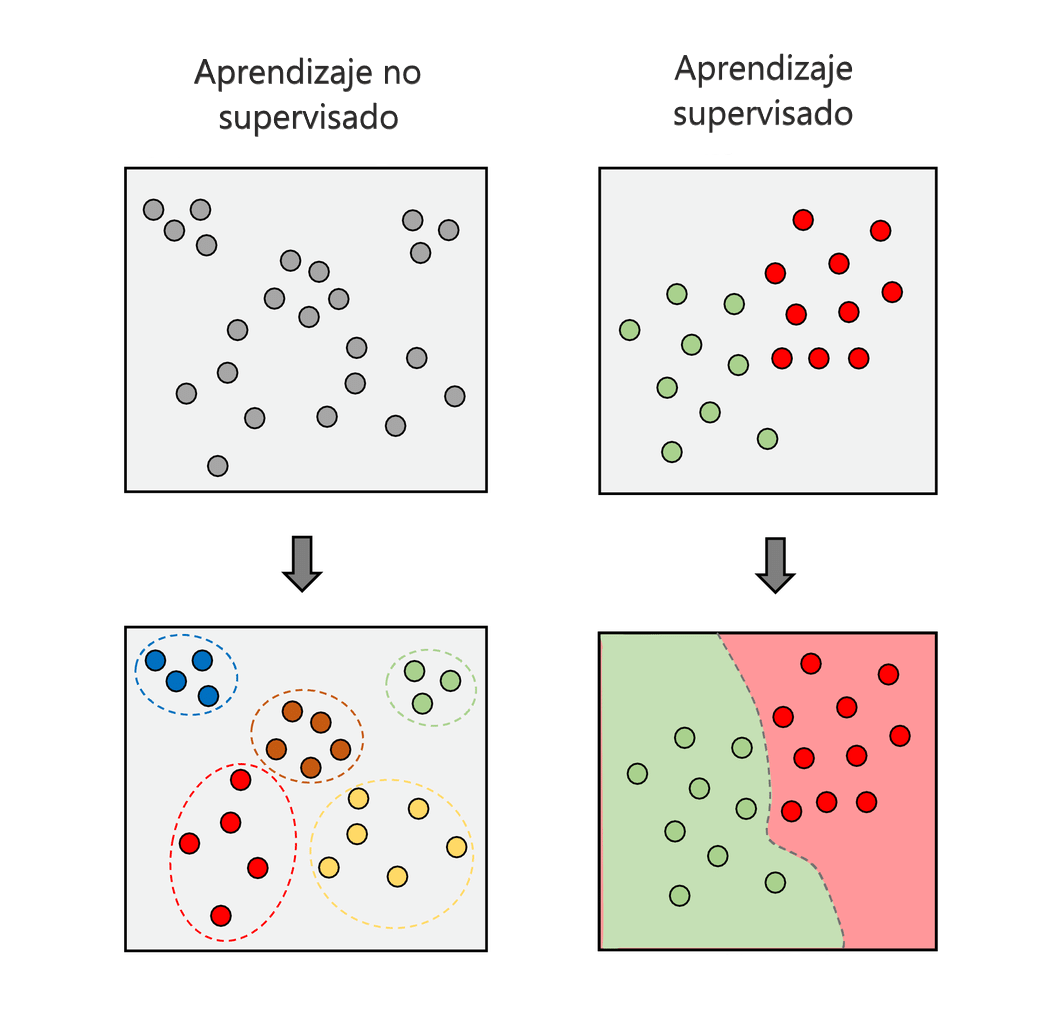
\includegraphics[width=7cm]{UL_vs_SL.png}
%		\end{center}
%	}
	\section{Agrupamiento}
	\frame[allowframebreaks]
	{
		\frametitle{Agrupamiento}
		\vspace{1em}
		Los algoritmos de agrupamiento conglomeran un conjunto de documentos en subconjuntos o cl\'usteres. Son utilizados para generar una estructura de categorías que se ajuste a un conjunto de observaciones. 
		
	\begin{center}
		\vspace{0.5em}
		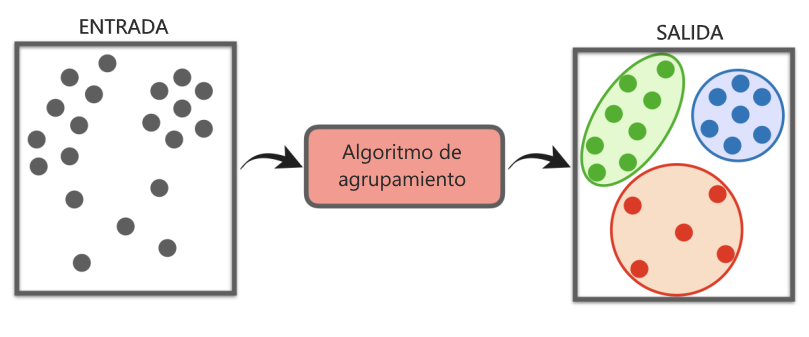
\includegraphics[width=10cm]{clustering_notion1.png}
	\end{center}
	}

	\frame{
		\frametitle{Caracter\'isticas generales}
		
		\vspace{4em}
		\begin{itemize}
			\item Es la forma más común de aprendizaje no supervisado.
			\item Los grupos formados deben tener un alto grado de asociación entre los documentos de un mismo grupo y un bajo grado entre miembros de diferentes grupos.
			\item La entrada clave para un algoritmo de agrupamiento es la medida de distancia. Diferentes medidas de distancia dan lugar a diferentes agrupamientos. 
		\end{itemize}
	}
	
	\frame{
		\frametitle{Hip\'otesis de agrupamiento}
		
		\vspace{5em}
		\textit{"Los documentos en el mismo grupo se comportan de manera similar con respecto a la relevancia para las necesidades de información."}
		
		\vspace{2em}
		La hipótesis establece que si hay un documento de un grupo que es relevante a una solicitud de búsqueda, entonces es probable que otros documentos del mismo clúster también sean relevantes. 
	}
	
	\frame{
		\frametitle{Clasificaci\'on de los algoritmos de agrupamiento}
		
		\vspace{5em}
		Seg\'un el tipo de estructura impuesta sobre los datos:
		\begin{itemize}
			\item \textit{agrupamiento particionado o plano} (flat clustering)
			\item \textit{agrupamiento jer\'arquico} (hierarchical clustering).
		\end{itemize}

	}

%	\frame{
%		\frametitle{Clasificaci\'on de los algoritmos de agrupamiento}
%		
%		\vspace{2.5em}
%		Seg\'un la pertenencia a los grupos:
%		\begin{itemize}
%			\item \textit{agrupamiento exclusivo o fuerte} (hard clustering): cada documento es miembro de exactamente un grupo.
%			\item \textit{agrupamiento difuso o suave} (soft clustering): un documento tiene membresía fraccionaria en varios grupos.
%		\end{itemize}
%		
%		\vspace{2em}
%		Seg\'un el tipo de estructura impuesta sobre los datos:
%		\begin{itemize}
%			\item \textit{agrupamiento particionado o plano} (flat clustering)
%			\item \textit{agrupamiento jer\'arquico} (hierarchical clustering).
%		\end{itemize}
%	}

%	\subsection{Medidas de similitud entre documentos}
%	\frame{
%		\frametitle{Medidas de similitud}
%		Sean $ d_{i} $ el $ i $-ésimo documento del corpus y $ w_{ik} $ el peso del t\'ermino $ k $ de un total $ N $ $ (N>0) $ en este documento.
%		
%		\begin{itemize}
%			\vspace{0.5em}
%			\item \textbf{Coeficiente de Dice:}
%			\begin{center}
%				$ S_{d_{i}, d_{j}} = \dfrac{2 \sum_{k=1}^{N} (w_{ik}w_{jk})}{\sum_{k=1}^{N}w_{ik}^{2} + \sum_{k=1}^{N}w_{jk}^{2}} $
%			\end{center}
%			
%			\vspace{0.5em}
%			\item \textbf{Coeficiente de Jaccard:}
%			\begin{center}
%				$ S_{d_{i}, d_{j}} = \dfrac{\sum_{k=1}^{N} (w_{ik}w_{jk})}{\sum_{k=1}^{N}w_{ik}^{2} + \sum_{k=1}^{max}w_{jk}^{2} - \sum_{k=1}^{N} (w_{ik}w_{jk})} $
%			\end{center}
%		
%			\vspace{0.5em}
%			\item \textbf{Coeficiente del coseno:}
%			\begin{center}
%				$ S_{d_{i}, d_{j}} = \dfrac{\sum_{k=1}^{N} (w_{ik}w_{jk})}{\sqrt{\sum_{k=1}^{N}w_{ik}^{2} \sum_{k=1}^{N}w_{jk}^{2}}} $
%			\end{center}
%		\end{itemize}
%	
%	}
	
%	\subsection{Medidas de evaluaci\'on}
%	\frame[allowframebreaks]
%	{
%		\frametitle{Medidas de evaluaci\'on}
%		\begin{itemize}
%			\vspace{5em}
%			\item \textbf{Pureza}
%			
%			\item \textbf{Información mutua normalizada}
%			
%			\item \textbf{\'Indice de Rand (Rand Index)}
%			
%			\item \textbf{Medida F} 
%		\end{itemize}	
%	}

	\subsection{Agrupamiento particionado}
	\frame
	{
		\frametitle{Agrupamiento particionado}
		\vspace{7em}
		El agrupamiento particionado crea un conjunto  de clústeres sin ninguna estructura explícita que los relacione entre sí. 
		
		El algoritmo m\'as importante de este tipo de agrupamiento es el K-means.
	}
	
%	\frame[allowframebreaks]
%	{
%		\frametitle{K-means}
%		\vspace{3em}
%		Es el algoritmo de agrupamiento particionado más importante. Su objetivo es minimizar la distancia euclidiana al cuadrado promedio entre los documentos y el centro de sus cl\'usteres. 
%		
%		El centro de un cl\'uster se define como la media o centroide $\mu$ de los documentos en un grupo $\omega$:
%		
%		\begin{center}
%			$ \overrightarrow{\mu}(\omega) \leftarrow \dfrac{1}{|\omega_{k}|} \sum_{\overrightarrow{x} \in \omega_{k}} \overrightarrow{x} $
%		\end{center}
%		
%		\framebreak
%		\textcolor{white}{.}
%		
%		\vspace{2em}
%		Una medida de qué tan bien los centroides representan a los miembros de su cl\'uster es la suma residual de cuadrados o RSS, que es la distancia al cuadrado de cada vector desde su centroide sumado sobre todos los vectores:
%		
%		\begin{center}
%			$ RSS_{k} = \sum_{\overrightarrow{x} \in \omega_{k}}|\overrightarrow{x} - \overrightarrow{\mu}(\omega_{k})|^2$
%			
%			\vspace{1em}
%			$ RSS = \sum_{k=1}^{K} RSS_{k} $
%		\end{center}
%		
%		RSS es entonces la función objetivo en K-means y nuestro objetivo es minimizarla.
%	
%	\framebreak
%	\textcolor{white}{.}
%	
%	\vspace{1em}
%	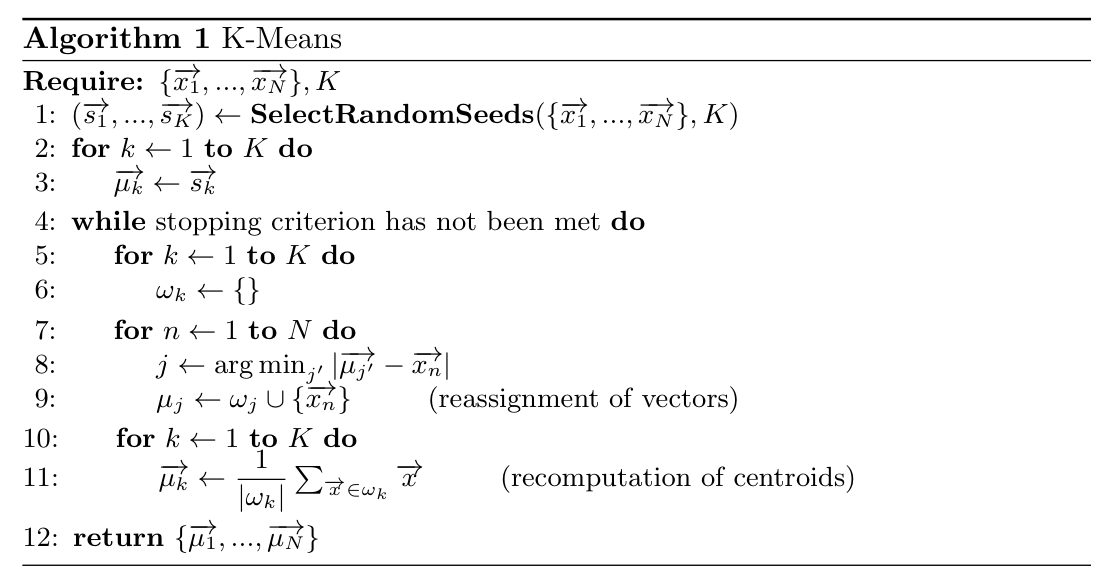
\includegraphics[width=10.5cm]{K-means.png}
%
%	\framebreak
%	
%	\textcolor{white}{.}
%	
%	\vspace{3em}
%	El primer paso de esta implementaci\'on de K-means es seleccionar al azar como centros iniciales de los cl\'usteres a K documentos, estas son las semillas. Luego, el algoritmo mueve los centros de los grupos en el espacio para minimizar el RSS. Este proceso se repite de manera iterativa hasta que se cumpla un criterio de parada.
%	
%%	\vspace{1em}
%%	Criterios de parada:
%%	\begin{itemize}
%%		\item Cuando se ha completado un número fijo de iteraciones I. 
%%		\item Cuando la asignación de documentos a grupos no cambia entre iteraciones.
%%		\item Cuando los centroides no cambian entre iteraciones.
%%		\item Cuando RSS cae por debajo de un umbral.
%%	\end{itemize}
%}

	\subsection{Agrupamiento jer\'arquico}
	\frame
	{
		\frametitle{Agrupamiento jer\'arquico}
		\vspace{2em}
		El agrupamiento jerárquico produce una jerarquía, una estructura que es más informativa que el conjunto no estructurado de clústeres devuelto por el agrupamiento particionado.
		
		\vspace{1em}
		Pueden tener dos enfoques: 
		\begin{itemize}
			\item De abajo hacia arriba (bottom-up) llamados de \textit{agrupamiento jer\'arquico aglomerativo}. 
			\item De arriba hacia abajo (top-down) conocidos como de \textit{agrupamiento jer\'arquico divisivo}. 
		\end{itemize}
	}
	
	
	\subsubsection{Agrupamiento jer\'arquico aglomerativo}
	\frame
	{
		\frametitle{Agrupamiento jer\'arquico aglomerativo}
		\vspace{3em}
		Los algoritmos de abajo hacia arriba tratan cada documento como un clúster único desde el principio y luego fusionan (o aglomeran) sucesivamente pares de grupos hasta que todos los grupos se han fusionado en uno solo que contiene todos los documentos. 
		Es por esto que se denomina agrupamiento jerárquico aglomerativo o HAC por sus siglas en ingl\'es. 
		
		\vspace{1em}
		Toman decisiones basadas en patrones locales sin tener inicialmente en cuenta la distribución global. Estas decisiones tempranas no se pueden deshacer.
	}

	\frame[allowframebreaks]
	{
		\frametitle{Medidas de similitud para cl\'usteres en HAC}
		
		\vspace{1em}
		\begin{itemize}
			\item \textbf{Agrupamiento por enlazamiento \'unico} (single link clustering): La similitud entre dos cl\'usters es la similitud de los dos objetos más cercanos entre ellos (mayor similitud).
	
			\item \textbf{Agrupamiento por enlazamiento completo} (complete link clustering): La similitud entre dos cl\'usters es la similitud de los dos objetos más alejados entre ellos (menor similitud). 
			
			\item \textbf{Agrupamiento aglomerativo por promedio de grupo} (group-average agglomerative clustering): Calcula la similitud promedio de todos los pares de documentos, incluidos los pares del mismo grupo, evitando así castigar valores extremos como en los criterios de enlace único y enlace completo.

			\item \textbf{Agrupamiento por centroide} (centroid clustering): La similitud de dos cl\'usters est\'a definida como la similitud de sus centroides.
		\end{itemize}
	
	}	
	
	\frame[allowframebreaks]
	{
		\frametitle{Algoritmo HAC}
		
		\vspace{1em}
		Dado un conjunto de N elementos a agrupar, el proceso básico del agrupamiento jerárquico aglomerativo es:
		\begin{enumerate}
			\item Se comienza con N cl\'usteres, resultado de asignar cada elemento al suyo propio. Se computa la matriz C de similitud de N×N.
			
			\item Se halla la similitud entre los pares de cl\'usteres con la medida deseada.
			
			\item Se toma el par más similar de clústeres y se combinan en un único clúster.
			
			\item Se calculan las similitudes entre el nuevo clúster y cada uno de los cl\'usteres antiguos.
			
			\item Se repiten los pasos 3 y 4 hasta que todos los elementos estén agrupados en un solo grupo de tamaño N.
		\end{enumerate}
	
	\framebreak
		\textcolor{white}{.}
	
	\vspace{0.9em}
	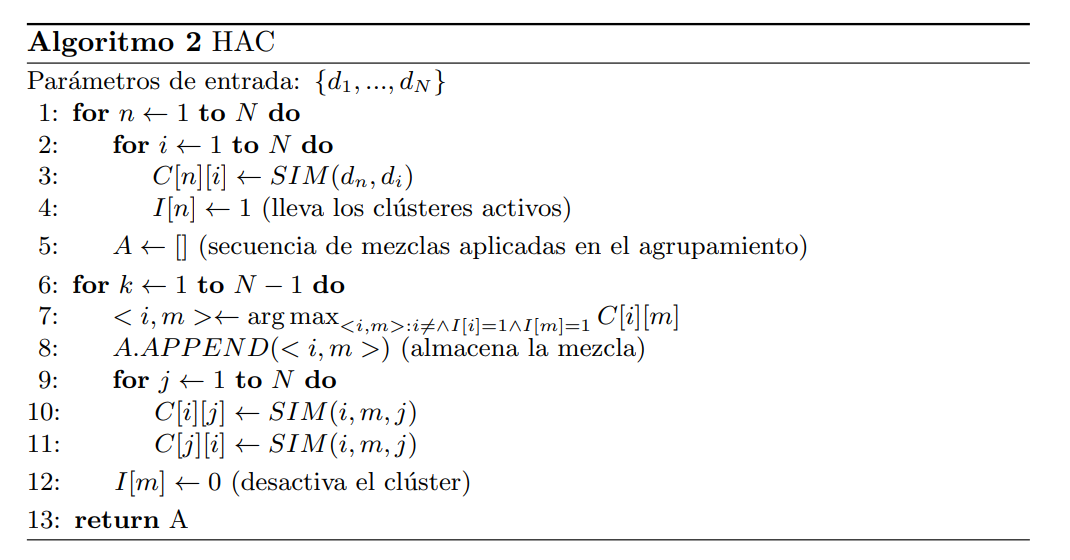
\includegraphics[width=10.5cm]{HAC.png}
	
	}	

	\subsubsection{Agrupamiento jer\'arquico divisivo}
	\frame
	{
		\vspace{4em}
		\frametitle{Agrupamiento jer\'arquico divisivo}
		Los algoritmos de arriba hacia abajo comienzan con todos los documentos en un grupo. El clúster se divide utilizando un algoritmo de agrupamiento particionado. Este procedimiento se aplica recursivamente hasta que cada documento está en su
		propio clúster.
		
		\vspace{0.5em}
		Se beneficia de la información completa sobre la distribución global al tomar decisiones de partición de alto nivel.
	}

	\subsection{Ventajas}
	\frame
	{
		\frametitle{Ventajas}
		\vspace{2.5em}
		\begin{itemize}
			\item No es necesario identificar las clases antes del procesamiento por lo que no se debe contar con expertos para este fin.
			
			\item Es útil para proporcionar estructura en grandes conjuntos de datos multivariados.
			
			\item Se ha descrito como una herramienta de descubrimiento porque tiene el potencial para revelar relaciones previamente no detectadas basadas en datos complejos.
			
			\item Debido a su amplia aplicación en dis\'imiles campos, cuenta el apoyo de una serie de paquetes de software, a menudo disponibles en la informática académica y otros entornos, por lo que se facilita su utilizaci\'on.
		\end{itemize}
	}

	\subsection{Desventajas}
	\frame
	{
		\frametitle{Desventajas}
		\vspace{6em}
		\begin{itemize}
			\item No se tiene una idea exacta de las clases creadas.
			\item No recibe retroalimentaci\'on.
		\end{itemize}
	}

	\subsection{Ejemplos de aplicaci\'on}
	\frame[allowframebreaks]
	{
		\frametitle{Ejemplos de aplicaci\'on en la web}
		\vspace{4em}
		Se ha utilizado en la recuperación de información para muchos propósitos diferentes:
		\begin{itemize}
			\item expansión de consultas
			\item agrupación e indexación de documentos
			\item visualización de resultados de búsqueda
		\end{itemize}
	
	 Permiten mejorar interfaz y experiencia de usuario y proporcionar una mayor eficacia o eficiencia del sistema de búsqueda. 
		
		\framebreak
		\textcolor{white}{.}
		
		\vspace{2em}
		\begin{itemize}
			\item \textbf{Agrupamiento de resultados de búsqueda} (Search result clustering): La presentación predeterminada de los resultados de búsqueda (documentos devueltos en respuesta a una consulta) en la recuperación de información es una lista sencilla. Los usuarios escanean la lista de arriba a abajo hasta que encuentran la información que buscan. 
			
			En su lugar, en la agrupación en clústeres de resultados de búsqueda los documentos similares aparecen juntos, siendo más fácil escanear algunos grupos coherentes que muchos documentos individuales. Esto es particularmente útil si un término de búsqueda tiene diferentes significados.
			
			\framebreak
			\textcolor{white}{.}
			
			\vspace{1em}
			\item \textbf{Dispersión-recopilación} (Scatter-Gather): Su objetivo es tambi\'en una mejor interfaz de usuario. Este agrupa toda la colección para obtener grupos de documentos que el usuario puede seleccionar o reunir manualmente. Los grupos seleccionados se fusionan y el conjunto resultante se vuelve a agrupar. Este proceso se repite hasta que se encuentre un grupo de interés.
			
			La navegación basada en la agrupaci\'on de clústeres es una alternativa interesante a la búsqueda por palabras clave, el paradigma de recuperación de información estándar. Esto es especialmente cierto en escenarios donde los usuarios prefieren navegar en lugar de buscar porque no están seguros de qué términos utilizar en la búsqueda.
			
			\framebreak
			\textcolor{white}{.}
			
			\item \textbf{Recuperaci\'on basada en cl\'usteres} (Cluster-based retrieval): La búsqueda en el modelo de espacio vectorial equivale a encontrar los vecinos más cercanos a la consulta. El índice invertido admite la búsqueda rápida del vecino más cercano para la configuración, sin embargo, a veces es posible que no se pueda usar un índice invertido de manera eficiente. En tales casos, se podr\'ia calcular la similitud de la consulta con cada documento, pero esto es lento. 
			
			La hipótesis de agrupamiento ofrece una alternativa: encontrar los cl\'usteres que están más cerca de la consulta y sólo considerar los documentos de estos. Como hay muchos menos clústeres que documentos, se disminuye grandemente el espacio de b\'usqueda. Adem\'as, los elementos que coinciden con una consulta son similares entre sí, por lo que tienden a estar en los mismos cl\'usteres, de esta forma la calidad no disminuye en gran medida.
		\end{itemize}
	}

	\section{Clasificaci\'on}
	\frame[allowframebreaks, c]
	{
		\frametitle{Clasificaci\'on}
		El problema de clasificaci\'on en sentido general consiste en determinar dentro de un conjunto de clases a cu\'al de ellas pertenece un objeto dado. En el marco de este documento es de inter\'es estudiar la clasificaci\'on de textos. 
		
		\framebreak
		
		Formas que requieren un alto esfuerzo humano:
		
		\begin{itemize}
			\item  Manualmente.
			\item  Uso de reglas (relacionado con las standing queries): Una regla captura una cierta combinaci\'on de palabras claves que identifican una clase.
		\end{itemize}
	
		
%		\textcolor{white}{.}
		
		\framebreak
		\textcolor{white}{.}
		
		Existe, sin embargo, un enfoque adicional a los dos anteriores mencionados. Este es el uso de \emph{Aprendizaje de M\'aquinas}. En este enfoque el conjunto de reglas de clasificaci\'on, o en general, el criterio usado para clasificar, es aprendido de forma autom\'atica a partir de los datos de entrenamiento.
		
		Al uso del Aprendizaje de M\'aquinas en la clasificaci\'on de textos se le conoce como \textbf{clasificaci\'on estad\'istica} de texto (o en ingl\'es \emph{statistical text classification}) si el m\'etodo de aprendizaje usado es estad\'itico.
		
		\framebreak
		
		Se presenta a continuaci\'on la definici\'on formal del problema de clasificaci\'on de textos, en el contexto del Aprendizaje de M\'aquinas.
		
		
		\textbf{Definici\'on 1:}
			Sea $\mathcal{{X}}$ el espacio de documentos y $\mathcal{C} := \{c_i \mid c_i \subset \mathcal{X}, i \in \{ 1,2,\dots,n\} \}$ un conjunto fijo de clases (tambi\'en llamadas categor\'ias o etiquetas). Sea adem\'as $D$ un conjunto entrenado de documentos clasificados $(d,c) \in \mathcal X \times \mathcal{C}$. El \emph{problema de la clasificaci\'on de textos} consiste en encontrar, usando m\'etodos o algoritmos de aprendizaje, una funci\'on \emph{clasificadora} $\gamma : \mathcal{X} \rightarrow \mathcal{C}$, que mapee documentos a clases, que satisfaga que $D \subset \gamma$. 	
		
		\framebreak
		
		\begin{itemize}
		\item  Estos expertos son  tambi\'en quienes determinan el conjunto de clases en que se clasificar\'an los textos. 
		\item Por ahora este trabajo se enfocar\'a nos enfocaremos en problemas en que cada documento se clasifica dentro de una sola clase.
		\item El aprendizaje que toma parte en la b\'usqueda de $\gamma$ es llamado \textbf{aprendizaje supervisado} debido a que se necesita la ayuda de uno o varios expertos que creen el conjunto de entrenamiento $D$.
		\end{itemize}
		
		\framebreak
	
}
	\subsection{Naive Bayes}
	\frame[allowframebreaks, c]{
		\frametitle{Naive Bayes}
		
		Uno de los m\'etodos m\'as comunes de aprendizaje supervisado es el conocido como \emph{Naive Bayes} (NB). Este es un m\'etodo de aprendizaje probabil\'istico.
		
		
		\framebreak
		 La probabilidad de un documento $d$ de pertenecer a una clase $c$ se puede expresar como $P(c\mid d)$. NB establece que la clase m\'as apropiada para un documento es la m\'as probable, o sea
		
		\[
		c_{map} = \argmax_{c\in\mathcal{C}} P(c \mid d).
		\]
		
		
		\framebreak
		
		
	
		Sin embargo la probabilidad condicional $P(c \mid d)$ es dif\'icil de determinar. Haciendo uso del \emph{Teorema de Bayes} la probabilidad anterior puede ser expresada como
		
		\[
		P(c \mid d) =\frac{ P(d\mid c) P(c)}{P(d)}.
		\]
		
		\framebreak
		
		\begin{itemize}
		\item El factor de normalizaci\'on $P(d)$ es usualmente ignorado ya que no aporta informaci\'on a la hora de buscar la clase m\'as apropiada para un documento $d$, ya que este tiene el mismo efecto en todos los candidatos. 
		\end{itemize}
		
		
Este c\'alculo puede ser simplificado si lo expresamos en funci\'on de los t\'erminos en los documentos. Supongamos que $\{t_1, t_2, \dots , t_n \}$ son los t\'erminos que aparecen en $d$. Entonces tenemos que  
		
		\[
		c_{map} = \argmax_{c\in\mathcal{C}} P(c) P(d \mid c) = \argmax_{c\in\mathcal{C}} P(c) \prod_{1\leq k\leq n} P(t_k \mid c),
		\]
		donde $P(t_k \mid c)$ es la probabilidad de que el t\'ermino $t_k$ aparezca en un documento de la clase $c$. 
		
		
		\framebreak
		
		Podemos considerar $p(t_k \mid c)$ como una medida de qu\'e tanto demuestra el t\'ermino $t_k$ que $c$ es la clase correcta. 
		
		\framebreak

		Para simplificar aun m\'as el c\'omputo se pueden sustituir los valores anteriores por sus logaritmos. Esto reducir\'a el costo de hacer los c\'alculos y adem\'as los errores aritm\'eticos, dado que la multiplicaci\'on se transforma en suma. La clase seleccionada ser\'ia entonces
		
		
		\[
		c_{map} = \argmax_{c\in\mathcal{C}} \left( \log(P(c))  + \sum_{1\leq k\leq n} \log(P(t_k\mid c)) \right).
		\]
		
		\framebreak
		
		
		Solo queda ver como se estiman los par\'ametros $P(c)$ y $P (t_k\mid c)$, dado que los valores reales no son posibles de calcular.
		
		
			Para la probabilidad previa se puede contar la frecuencia relativa de cada clase en $D$:
		
		\[P(c) = \frac{ N_c }{N} , \]
		donde $N_c$ es el n\'umero de documentos en la clase $c$ y $N$ es el n\'umero total de documentos.
		
		\framebreak
		
		 Se procede de manera similar para la probabilidad espec\'ifica de una palabra en una clase
		\[
		P(t_k\mid c) =\frac{ T_{c,t_k}}{T_{c}},
		\]
		
		
		
		donde $T_{c,t_k}$ indica la cantidad de veces que ocurre  la palabra $t_k$ en todos los documentos de la clase $c$ y $T_{c}$ es la cantidad total de palabras (contando repeticiones) en toda la clase $c$. 
		
		\framebreak
		
		Sin embargo, a\'un tenemos un problema con estas f\'ormulas y es que estamos asignando \textbf{probabilidad cero a todos las clases que no contengan a todas las palabras del documento a clasificar}. Para evitar esto adicionamos por defecto una unidad a cada contador lo cual es conocido como \emph{Laplace smoothing}
		\[
		P(t\mid c) = \frac{T_{c,t} + 1}{T_c + |V|},	
		\]
		donde $|V|$ es el n\'umero total de t\'eminos en el vocabulario.
		
		Es importante destacar que en este m\'etodo se est\'a obviando la posici\'on de las palabras.
		
		
		\framebreak
		
		
		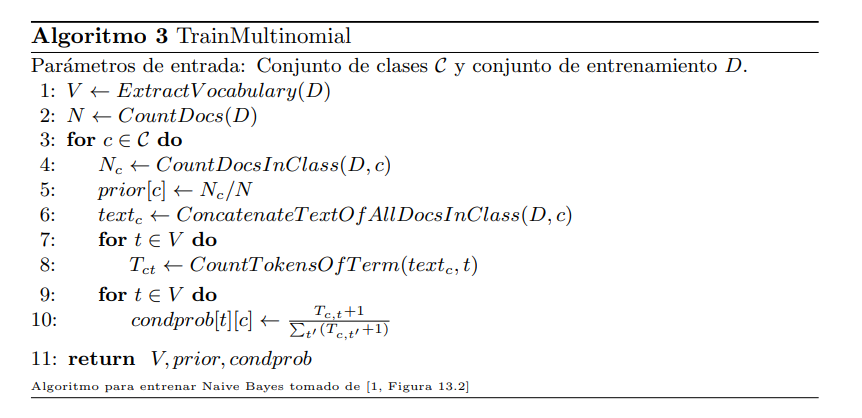
\includegraphics[width=10.5cm]{TrainMultinomial.png}
		
		\framebreak
		
		
		
		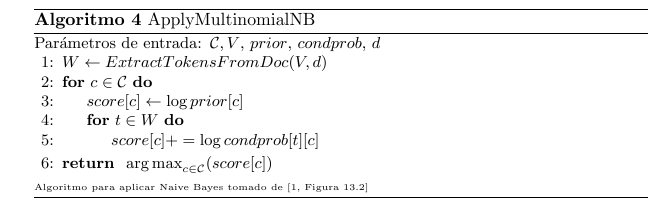
\includegraphics[width=10.5cm]{ApplyMN.png}
		
		
		\framebreak
		
		Podemos deducir de los algoritmos que la complejidad de ambos es linear en el tiempo que toma escanear la informaci\'on. Dado que esto hay que hacerlo al menos una vez, se puede decir que este m\'etodo tiene complejidad temporal \'optima. Dicha eficiencia hace que NB sea un m\'etodo de clasificaci\'on tan usado.
	}

	\subsection{Feature Selection}
	\frame[allowframebreaks, c]{
		\frametitle{Feature Selection}
		
		Un t\'ermino con ruido (\emph{noise feature}) es aquel que al pertenecer a la representaci\'on de los documentos, provoca un aumento del error de clasificaci\'on de los datos.
		
	\framebreak
	
		La selecci\'on de t\'erminos consiste en reducir el vocabulario, considerado en la clasificaci\'on de textos solo un subconjunto del que aparece en el conjunto de entrenamiento. N\'otese que, al disminuir el tama\~no del vocabulario aumenta la eficiencia de los m\'etodos de entrenamiento y clasificaci\'on (aunque no es el caso de NB).
		
	\framebreak
				
%		Selecci\'on de t\'erminos prefiere un clasificador m\'as simple antes que uno m\'as complejo. Esto es \'util cuando el conjunto de entrenamiento no es muy grande.
		
		%		Nos concentraremos en describir la Selecci\'on de t\'erminos para la clasificaci\'on de dos clases.
		
		\begin{itemize}
		\item En FS usualmente se fija una cantidad $k$ de vocablos por cada clase $c$, que ser\'an los usados por el clasificador. 
		
		\item Para seleccionar los $k$ t\'erminos deseados se establece un ranking entre los t\'erminos de la clase, haciendo uso de una funci\'on de medida de utilidad $A(t,c)$, y luego se escogen los $k$ mejor posicionados. 
		
		\end{itemize}
%		El algoritmo b\'asico consiste en para cada clase $c$ iterar por todos los t\'erminos del vocabulario y computar su medida de utilidad para la clase; para finalmente ordenar los resultados y devolver una lista con los $k$ mejores.
		
		\framebreak
		Se presenta a continuaci\'on tres de los m\'etodos de calcular $A(t,c)$ m\'as comunes.
		
		\begin{itemize}
			\item\textbf{Informaci\'on Mutua.}
			\smallskip
			
			Computar $A(t,c)$ como el valor esperado de informaci\'on mutua (\emph{Mutual Information} (MI)), da una medida de \textbf{cu\'anta informaci\'on aporta, la presencia en $c$ de un t\'ermino dado, a tomar la decisi\'on correcta de clasificaci\'on de un documento. }
			\[
			I(U_t;C_t) = \sum_{e_t \in \{ 1,0 \} } \sum_{e_c \in \{ 1,0 \} } P( U_t = e_t, C_t = e_c) \log_2 \frac{P (U_t = e_t, C_t = e_c) }{ P(U_t = e_t) P(C_t = e_c) },
			\]
			donde $U_t$ es una variable aleatoria que toma valor $e_t = 1$ si el documento contiene el t\'ermino $t$ y $e_t = 0$ en otro caso, y $C$ es otra variable aleatoria que toma valor $e_c = 1$ si el documento est\'a en la clase $c$ y $e_c = 0  $ en otro caso. 
			
			\smallskip
			
%		\framebreak
%			
%			MI mide cu\'anta informaci\'on un t\'ermino contiene acerca de una clase. Por tanto, mantener los t\'erminos que est\'an cargados de informaci\'on, y eliminar los que no, contribuye a reducir el ruido y mejorar la precisi\'on del clasificador.
%			
%			\smallskip
			
		\framebreak
			
			\item\textbf{Selecci\'on Chi cuadrado $\chi^2$.} 
			\smallskip
			
			El test $\chi^2$ se usa para medir el grado de independencia de los eventos: \textbf{ocurrencia de los t\'erminos y ocurrencia de las clases. }
			
			\[
			\chi^2(D,t,c) = \sum_{e_t\in \{ 1, 0 \}} \sum_{e_c\in \{ 1, 0 \}} \frac{(N_{e_te_c} - E_{e_t e_c}) ^2 } { E_{e_t e_c}},
			\]
			donde $N$ es la frecuencia seg\'un $D$, $E$ es la frecuencia esperada y $e_t$ y  $e_c$ se definen como en la medida anterior.
			
			\smallskip
			
		\framebreak
		
			\item \textbf{Selecci\'on basada en frecuencia}.
			\smallskip
			
			Esta medida consiste en priorizar los t\'erminos que son m\'as comunes en la  clase. Puede ser calculada de dos formas diferentes. La primera es\textbf{ cantidad de repeticiones de un t\'ermino en los documentos de una clase}, conocida como \textbf{frecuencia en colecci\'on}. La otra es \textbf{frecuencia de documentos}, y se calcula como la \textbf{cantidad de documentos en la clase que contienen al t\'ermino en cuesti\'on.}
			
%			\smallskip
%			
%			Cuando son seleccionados varios miles de t\'erminos, entonces esta medida es bastante buena. Esta es preferible a otros m\'etodos m\'as complejos cuando se aceptan soluciones sub\'optimas.
			
		\end{itemize}
		
		
	}

	\subsection{K Nearest Neighbor}
	\frame[allowframebreaks, c]
	{
		\frametitle{K Nearest Neighbor}
				
		
			El m\'etodo que ser\'a presentado en esta secci\'on, as\'i como otros similares, asignan a cada t\'ermino cierto valor de importancia relativa al documento en que aparece. Para esto se cambia la representaci\'on de los documentos a vectores de $\mathbb{R}^{|V|}$, donde a cada componente corresponde cierto peso que se le asigna al t\'ermino correspondiente a esta. Entonces, el espacio de documentos $\mathcal{X}$ (dominio de $\gamma$) es $\mathbb{R}^{|V|}$. A esta forma de representaci\'on de documentos se le conoce como \textbf{modelo de espacio de vectores}.
			
		\framebreak		
			
			\textbf{Hip\'otesis de contig\"uidad:} Documentos en la misma clase forman una regi\'on contigua  y regiones de diferentes clases no se superponen.
			
		\framebreak	
				
			Las decisiones de muchos clasificadores basados en espacio de vectores dependen de una noci\'on de distancia. Pueden ser usadas por ejemplo similitud basado en el coseno (del \'angulo formado entre los vectores) o distancia Euclideana. Por lo general, no hay mucha diferencia entre usar una u otra de estas distancias.
			
		\framebreak	
						
			La tarea de la clasificaci\'on en el modelo de espacio de vectores es determinar las fronteras entre los documentos pertenecientes a una u otra clase. Estas \'ultimas son llamadas \textbf{ fronteras de decisi\'on} ya que dividen el espacio en diferentes poliedros, tales que si un documento pertenece a uno determinado, autom\'aticamente sabemos de qu\'e clase es. 
			
		\framebreak	
						
			En K Nearest Neighbor la frontera de decisi\'on se determina localmente. En este se asigna cada documento a la misma clase que la mayor\'ia de los $k$ puntos m\'as cercanos al documento. Basado en la hip\'otesis de contig\"uidad se espera que el documento $d$ pertenezca a la misma clase que aquellos m\'as cercanos a \'el.
			
%		\framebreak	
%						
%			En $kNN$ para subdividir el espacio de documentos en regiones, dado un $k \in \mathbb{N}$ fijo, consideramos cada regi\'on como el conjunto de puntos para los cuales los $k$ puntos m\'as cercanos son los mismos. Estas regiones son poliedros convexos. Luego para cada una de estas regiones existe una clase a la que pertenecen todos sus puntos, que es aquella a la que pertenecen la mayor\'ia de los documentos, ya clasificados, que est\'an dentro de la regi\'on. En caso de que haya empate, la decisi\'on de a que clase asignar a un nuevo documento que pertenece a esta regi\'on del espacio, es tomada aleatoriamente entre las clases empatadas.
			
		\framebreak
			
			
			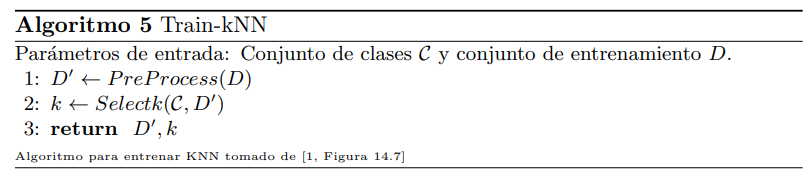
\includegraphics[width=10.5cm]{TrainkNN.png}
			
		\framebreak
			
			
			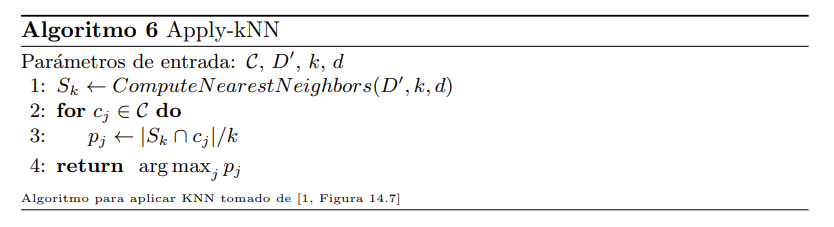
\includegraphics[width=10.5cm]{ApplykNN.png}
			
		\framebreak
			
			El par\'ametro $k$ es usualmente seleccionado basado en el conocimiento que se posee sobre los problemas de clasificaci\'on similares al que se tiene. Otra forma de seleccionar $k$ es usando conjuntos de documentos de prueba (ya clasificados) para ver qu\'e valor de $k$ producen mejores resultados.
			
%		\framebreak	
%						
%			Tambi\'en hay variantes del m\'etodo donde lo que se hace es calcular una similitud entre el documento $d$ a clasificar y cada uno de los $k$ m\'as cercanos, usando, por ejemplo, el coseno entre los vectores. Luego se hace un ranking entre las clases a las que pertenecen cada uno de los $k$ puntos. Para ello se calcula para cada $c$, la suma de la similitud entre $d$ y cada uno de los puntos que pertenecen a $c$ y a la vez est\'an entre los $k$ mencionados. La siguiente funci\'on $score$ produce el resultado deseado
%			\[
%			score(c,d)  = \sum_{d'\in S_k(d)} I_c(d') \cos(\overrightarrow{v}(d'),\overrightarrow{v}(d)),
%			\]
%			donde $S_k(d)$ es el conjunto de los $k$ puntos m\'as cercanos a $d$ e $I_c(d')$ es $1$ o $0$ en dependencia de si $d'$ pertenece a la clase $c$ o no. Finalmente se selecciona para $d$ la clase $c$ que m\'as alto aparezca en el ranking. En ocasiones esta variante presenta mayor exactitud que la anterior.
%			
	}
	
	\subsection{Medidas de evaluaci\'on}
	\frame[allowframebreaks, c]
	{
		\frametitle{Medidas de evaluaci\'on}
			Una alta exactitud en la clasificaci\'on de los datos de entrenamiento no necesariamente se traduce en resultados correctos en los nuevos documentos introducidos. Puede suceder que el sistema resulte sobreentrenado (\emph{over-fitting}) o subentrenado (\emph{under-fitting}).

		\framebreak	
			
			 El primero de estos ocurre cuando un sistema se entrena demasiado o se entrena con datos extra\~nos. En este caso el algoritmo de aprendizaje puede quedar ajustado a unas caracter\'isticas muy espec\'ificas de los datos de entrenamiento que no tienen relaci\'on causal con la funci\'on objetivo. Entonces el clasificador puede aprende incorrectamente a clasificar los elementos de alguna clase.
			 
			  Por otro lado under-fitting ocurre cuando el sistema tiene informaci\'on muy vaga sobre la frontera entre clases lo que provoca cierta aleatoriedad en la clasificaci\'on.

		\framebreak	
			
			Para evaluar la labor de un clasificador se debe emplear un conjunto de documentos diferente al conjunto entrenante el cual se llama conjunto de prueba. Este debe estar en todo momento aislado del conjunto de entrenamiento. Usualmente los datos que se tienen se dividen entre el conjunto entrenante y de prueba a raz\'on de $4:1$.

		\framebreak	
			
			Las siguientes tres m\'etricas pueden ser utilizadas para evaluar clasificadores de dos clases (c y \~c):	
			
			\begin{itemize}
				
		\framebreak	
				\item\textbf{Precisi\'on}
				\[
				Precision = \frac{tp}{tp + fp},
				\]
				
				donde $tp$ es el n\'umero de documentos clasificados correctamente como de $c$ y $tp + fp$ es el total de documentos clasificados como $c$.
				
		\framebreak	
				\item\textbf{Recobrado}
				\[
					Recobrado = \frac{tp}{tp + fn},
				\]
				donde $tp$ es el n\'umero de documentos correctamente identificados como $c$ y $tp + fn$ es el n\'umero de documentos que pertenecen a $c$.
				
				
		\framebreak	
				\item\textbf{Medida $F$} 
				$$
				F = 2 \times  \frac{Precision \times Recobrado}{Precision + Recobrado}
				$$
			\end{itemize}
			
			
			
		\framebreak	
			
			Podemos ver las clasificaciones anteriores en la matriz de contingencia. 
			
			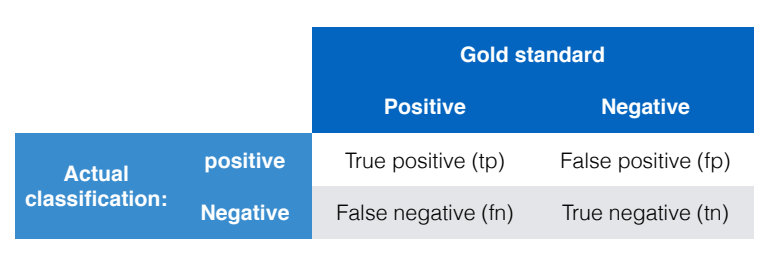
\includegraphics[width=10.5cm]{Tabla.png}
			
		\framebreak	
					
			En el caso que la cantidad de clases sea mayor que dos, podemos computar promedios entre las m\'etricas anteriores viendo el clasificador como uno de dos clases aplicado a cada clase $c$ (y su complemento). Existen dos promedios que son los m\'as usados para esto. Macropromedio calcula simplemente la media entre las medidas anteriores para cada clasificador de dos clases. Micropromedio primero adiciona las matrices de contingencia correspondientes a diferentes clases y luego aplica una de las m\'etricas anteriores sobre la matriz resultante. 
			
				
	}
	
	\subsection{Ventajas}
	\frame[allowframebreaks, c]
	{
		\frametitle{Ventajas}
		
		\textbf{Ventajas:}
		\begin{itemize}
			\item Al usar el aprendizaje supervisado se puede tener una idea exacta sobre las clases de los documentos, dado que estas se crean en base a caracter\'isticas expl\'icitas de los mismos. 
			\item La salida suele ser m\'as precisa que en el aprendizaje supervisado
			\item El proceso es f\'acil de comprender ya que las acciones de la m\'aquina se reconocen con precisi\'on.
			\item Es m\'as facil de trabajar con el aprendizaje supervisado que con el no supervisado. 
			\item Se eval\'ua y recibe retroalimentaci\'on para comprobar la correctitud. 
		\end{itemize}
	}
	
	\subsection{Desventajas}
	\frame[allowframebreaks, c]
	{
		\frametitle{Desventajas}
		
			\textbf{Desventajas:}
			\begin{itemize}
				\item Se necesita un especialista que determine cu\'ales ser\'an las clases en que se desea clasificar.
				\item Se requiere de un conjunto de datos entrenantes.
				\item Por lo general no se resuelven tareas tan complejas como en el aprendizaje supervisado.
				\item Los algoritmos solo funcionan dentro de las restricciones que se le han impuestos por lo que no proporcionan soluciones creativas.
				\item Suelen requerir mucho tiempo de entrenamiento.
				\item Puede predecir la salida incorrecta si los datos de prueba son diferentes de los datos de entrenamiento.
			\end{itemize}
	}
	
	\subsection{Aplicaciones en la Recuperaci\'on de la Informaci\'on}
	\frame[allowframebreaks, c]
	{
		\frametitle{Aplicaciones en la Recuperaci\'on de la Informaci\'on}
		
		
		\begin{itemize}

		\item Recuperaci\'on de consultas permanentes.

		\framebreak	
			
			\item La organizaci\'on del correo personal: Es otros de los ejemplos relacionados con la Web que pueden ser resueltos mediante clasificaci\'on. En muchas ocasiones una persona tiene un n\'umero grande de correos en el buz\'on de entrada. A la hora de revisarlo ser\'ia deseable que pudiera dirigirse directamente a aquellos que son de inter\'es para \'el. Para ello la organizaci\'on autom\'atica del correo en carpetas podr\'ia ser una ventaja invaluable. Un ejemplo particular ser\'ia la carpeta de correo spam.

		\framebreak	
			
		\item Clasificaci\'on de valoraciones sobre algo en positivas o negativas: Esto tendr\'ia numerosas aplicaciones pr\'acticas como pudiera ser la selecci\'on de una pel\'icula. Un usuario podr\'ia revisar la cantidad de comentarios negativos, antes de lanzarse a disponer de dos horas de su tiempo viendo un material audiovisual que no resultar\'a muy placentero. Los sistema que se especializan en este tipo de sugerencias de contenido, son llamados usualmente \textbf{sistemas de recomendaci\'on}.

		\framebreak	
			
		\item	La clasificaci\'on de documentos en t\'opicos: Esta clasificaci\'on facilitar\'ia la implementaci\'on de un \textbf{motor de b\'usqueda vertical}, que permita al usuario restringir su b\'usqueda al tema deseado. Un SRI con semejante caracter\'istica permite hacer una b\'usqueda m\'as precisa en las consultas m\'as especializadas por el usuario.
			
		\framebreak				
			
		\item Creaci\'on de \'indices de los contenidos almacenados en un SRI: En el proceso de creaci\'on de los mencionados \'indices la clasificaci\'on puede jugar un importante papel. Por citar algunos ejemplos puede usarse para detectar el lenguaje de un documento, la segmentaci\'on y capitalizaci\'on de las palabras y el codificado del documento.
			
	\end{itemize}	
	}
	
	\subsection{Otros ejemplos de aplicaci\'on}
	\frame[allowframebreaks, c]
	{
		\frametitle{Otros ejemplos de aplicaci\'on}
		
		\begin{itemize}

		\item La bioinform\'atica: Con el uso de sus algoritmos se permite automatizar la b\'usqueda de patrones en conjuntos de datos, que puedan ayudar a entender diferentes procesos biol\'ogicos que se manifiestan en los mismos. Debido a los grandes vol\'umenes de datos que se tienen ha crecido mucho en los \'ultimos a\~nos la aplicaci\'on de la clasificaci\'on en esta disciplina.
		
		
		\framebreak		
			
		\begin{itemize}
			
			\item Predicci\'on de gen. Esta consiste en determinar que fracciones de una secuencia de ADN codifican prote\'inas. 
			
			\item Investigaci\'on de comunidades de microbios en nichos ecol\'ogicos. As\'i se puede obtener informaci\'on taxon\'omica y metab\'olica de las comunidades estudiadas. 
			
			\item Prote\'omica
			
			\item Microarrays 
			
			\item La biolog\'ia de sistemas.
		
		\end{itemize}
		
		\framebreak			
		
		\item Reconocimiento de algunos rasgos distintivos de una persona, como pueden ser, reconocimiento de rostros, huellas o voz. Este \'ultimo lo tenemos al alcance de nuestras manos en asistentes virtuales como Siri o  Google. Estas aplicaciones se entrenan para reconocer caracter\'isticas distintivas de tu voz, mediante un proceso de aprendizaje supervisado, para luego poder diferencias c\'uando eres t\'u quien les est\'a hablando.
		
		\framebreak			
		
		\item El mercado financiero: Se puede emplear en mejorar el mercado digital, las ventas en l\'inea, identificar el valor de vida \'util de un cliente, la tasa de abandono, recomendaciones de productos y an\'alisis de impacto de campa\~nas de mercado.
		
		\framebreak	
				
		\item En la seguridad inform\'atica: acciones como detecci\'on de virus, enlaces maliciosos y fraude. 
		\item Internet de las cosas (IoT).
		
		\item Los motores de recomendaci\'on 
		\item La fijaci\'on de precios din\'amicos de productos.
		
		\end{itemize}
	}

%	\section{Conclusiones}
%	\frame
%	{
%		\frametitle{Conclusiones}
%	}
%
%	\section{Referencias}
%	\frame
%	{
%		\frametitle{Referencias}
%	}
\end{document} 